\section[Datenassimilation]{4D- Datenassimilation}
\begin{frame}[<+->]
\frametitle{4D- Datenassimilation}
    \begin{itemize}
     \item Benutzt im Kontext der numerischen Wettervorhersage und ozeanographischen Modellen
     \item Eingeführt von Talagrand und Dimet $\approx$ 1986 (\cite{dimet1986variational})
     \item Ziel: Annäherung eines Modells an Observierungsparameter durch Steuerungsparameter um über $T$ hinaus zu extrapolieren
%      \item Wendet Methoden der optimalen Steuerung auf die Datenassimilation an
    \end{itemize}

\end{frame}

\begin{frame}
\frametitle{4D- Datenassimilation}
    \begin{block}{Voraussetzung}
    \parbox[c][3.5\baselineskip][t]{\textwidth}{
    \begin{itemize}
     \item $\dot{x} = F(x),~ x_0 = x(0),~F\in C^1(\R^n)$
%      \item $x_{obs}(t)$ - Observierungsparameter (Funktion oder diskrete Werte)
%      \item $C$ - Projektion von $X_{\text{State}}$ nach $X_{\text{Obs}}$ 
    \end{itemize}
    }
    \end{block}
   \begin{block}{Problem}
      \begin{tikzpicture}
     \begin{axis}[width=12cm,height=5cm,xlabel=t,ylabel=x] 
     \addplot[blue,domain=0:10,samples=100]{sin(deg(x))};
  \legend{$x$}
     \end{axis}
   \end{tikzpicture}
   \end{block}
\end{frame}
\begin{frame}
\frametitle{4D- Datenassimilation}
    \begin{block}{Voraussetzung}
    \parbox[c][3.5\baselineskip][t]{\textwidth}{
     \begin{itemize}
     \item $\dot{x} = F(x),~ x_0 = x(0),~F\in C^1(\R^n)$
     \item $x_{obs}(t)$ - Observierungsparameter (Funktion oder diskrete Werte)
%      \item $C$ - Projektion von $X_{\text{State}}$ nach $X_{\text{Obs}}$ 
    \end{itemize}
    } 
   \end{block}
   \begin{block}{Problem}
      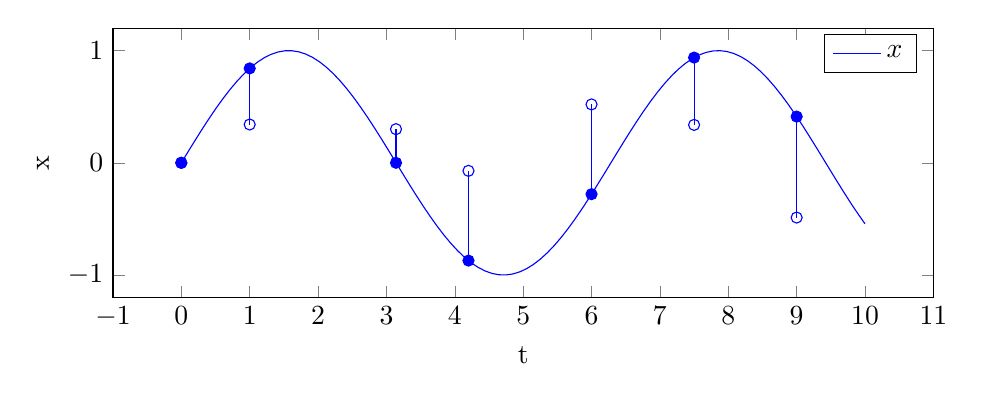
\begin{tikzpicture}
     \begin{axis}[width=12cm,height=5cm,xlabel=t,ylabel=x] 
     \addplot[blue,domain=0:10,samples=100]{sin(deg(x))};
     \addplot+[blue,draw=none,mark=*, mark options={blue},error bars/.cd, y dir=plus,y explicit,error mark=o,error mark options={blue,mark size=2pt}] 
     coordinates { 
      (0,0) +- (0,0) 
     (1,0.8415) +- (0.5,-0.5) 
     (3.14,0) +- (0.05,0.3) 
     (4.2,-0.8715) +- (0,0.8)
     (6.0,-0.27942) +- (0,0.8)
     (7.5,0.93799) +- (0.1,-0.6) 
     (9,0.41212) +- (0.3,-0.9)}; 
  \legend{$x$}
     \end{axis}
   \end{tikzpicture}
   \end{block}
\end{frame}



\begin{frame}[<+->]
  \frametitle{Datenassimilation Schritte}
	\begin{block}{Ziel: Minimiere Kostenfunktional}
	\begin{equation}\label{eq:costFunctional}
		\min_{x_o} J(x_0) = \min_{x_o} \frac{1}{2}\int_0^T \|Cx(t) - x_{Obs}(t)\|^2dt
	\end{equation}
	  $C$ - Projektion von $X_{\text{State}}$ nach $X_{\text{Obs}}$ 
	\end{block}
	\begin{block}{Datenassimilation Schritte}
	\begin{enumerate}
	 \item Berechnung Kostenfunktional
	 \item Berechnung $\nabla J(x_0)$
	 \item Optimierung
	\end{enumerate}
	\end{block}
\end{frame}
 
\begin{frame}[<+->]
  \frametitle{Datenassimilation Schritte}
  \begin{block}{Lösen einer ODE - z.B. Implizite Mittelpunktsregel(IMP)}
	\begin{equation}
	 x_n = x_a + h F \left(0.5 (x_a + x_n), t + 0.5 h\right)
	\end{equation}
	Speichere Werte $x_i$, berechne $J(x_0)$ mittels numerischer Quadratur
  \end{block}
  \begin{block}{Berechnung des Gradienten $\nabla J(x_0)$}
	Integriere das inhomogene adjungierte Tangent Linear Model rückwärts in $t$
	\begin{equation}
	  \dot{ \bar{x}}(t) =  -\frac{\partial F(x(t))}{\partial x}^\tr \bar x(t) +C^\tr(Cx(t) - x_{\text{obs}}(t)), ~ \bar x(T) =0
	\end{equation}
	\[
	\text{mit }\nabla J(x_0) = -\bar x(0)
	\]
  \end{block}
  \begin{block}{Optimierung}
	Optimiere mit einem geeigneten Verfahren (z.B. BFGS)
  \end{block}

\end{frame} 

\begin{frame}[<+->]
  \frametitle{Problemstellung}
  \begin{block}{Problemstellung}
  \centering
	Wie kann die Datenassimilation für den Fall
	\[
	  \dot{x} = F(x),~ x_0 = x(0),~F\in C^{0,1}(\R^n)
	\]
	betrachtet werden?
  \end{block}
\end{frame} 
